\documentclass{article}
\usepackage[utf8]{inputenc}
\usepackage[english]{babel}
\usepackage{graphicx}
\usepackage{geometry}
\usepackage{float}
\usepackage{helvet}
\usepackage[backend=bibtex, bibencoding=ascii]{biblatex}
\usepackage{csquotes}
\renewcommand{\familydefault}{\sfdefault}
\AtEveryBibitem{\clearlist{abstract}}
\geometry{
	left=1in,
	right=1in,
	top=.0075in,
	bottom=.45in
}

\usepackage{multicol}
\setlength{\columnsep}{1cm}

\title{\fontfamily{phv}\textbf{Exploring New Approaches to Interactive Rendering Utilizing Pixel Synchronization}}
\author{Bryan Pawlowski, Professor Mike Bailey \\ \textit{Oregon State University}\vspace{-2ex}}
\date{\vspace{-5ex}}

\bibliography{database.bib}

\begin{document}
\vspace{-3ex}
\maketitle
\pagenumbering{gobble}
\begin{figure}[H]
	\centering
	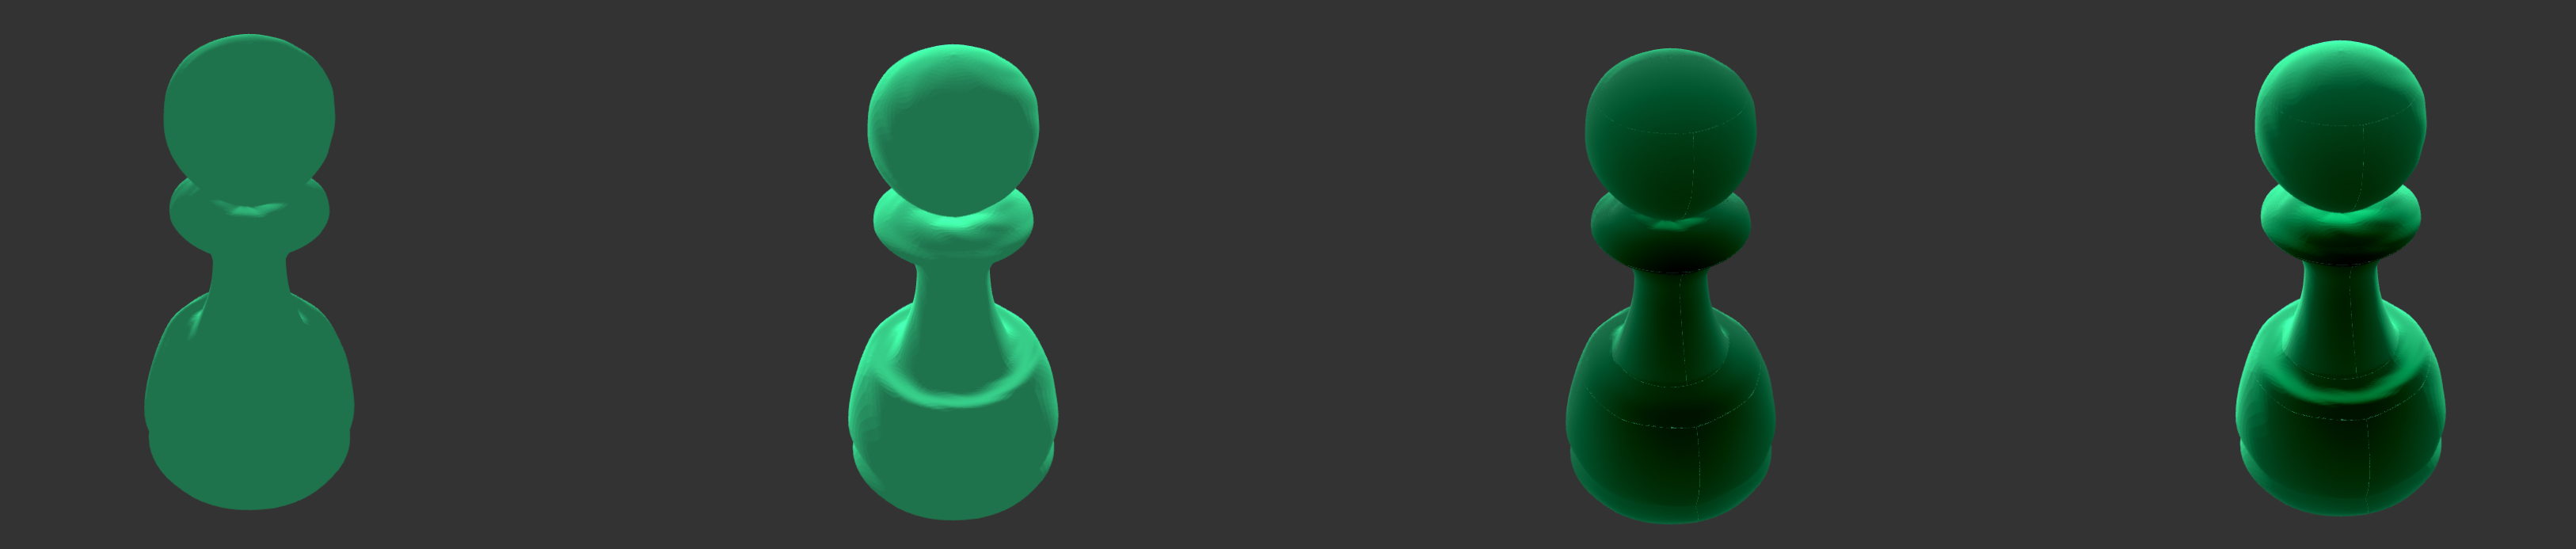
\includegraphics[width=1.0\textwidth]{Result.png}
	\caption{\textit{From left to right, Phong Smooth Shading, Phong with Normal Wrapping, Phong with Pixel Sync Depth Map, then Phong with a combination of Smooth Shading and Pixel Sync Depth Map.}}
	\label{fig: ResultPhotos}
\end{figure}

\begin{multicols*}{2}  

\section*{\fontfamily{phv}\textbf{Introduction}}

\vspace{-1ex}

In the early stages of graphics programming, we had a very basic job to do in
the eyes of the GPU. We were to give the GPU information on the 3D object, set
various contexts and modes, then told it to draw. Once these fixed-function
GPUs began to draw, our influence on the GPU was over. Later on, we were given
the ability to program the GPU's pipeline stages; starting first with a
programmable vertex and fragment/pixel shader, then getting increasingly
complex. The advent of programmable shaders gave graphics programmers the
chance to unlock the GPU's potential to render a large number of what the
programmer could think of. However, there remained the issue that we couldn't
program the GPU to take advantage of any types of syncronization constructs.
Since the main advantage of a GPU is to produce spectacular images quickly, it
makes sense why synchronization was never really factored into a Graphics
Processor's architecture, until now.\\ \\  With the advent of hardware support
of Pixel Synchronization, programmers are given the ability to put a barrier
into shader code which orders pixels being processed. Given this new
capability, we are now able to build knowledge of entire objects with fewer
passes, when coupled with the use of Unordered Access Views. Since UAVs are
shared between all pixels in flight, a programmer used to have no way of
guaranteeing against data races. With the addition of Pixel Synchronization,
we are now able to guarantee that parts of the UAV will be accessed in a
deterministic order. When pixel ordering is invoked within the pixel shader, a
barrier based on screen space is created. What this means is that each pixel
in flight at the same screen position hits a barrier, is ordered based upon
primitive, then executed in-order.

\noindent\makebox[\linewidth]{\rule{\columnwidth}{0.4pt}}

\section*{\fontfamily{phv}\textbf{My Work}}

\vspace{-1ex}

The main purpose of my work is to answer the question of how this Pixel
Synchronization hardware capability is can be utilized to enhance existing
render techniques. This work is important to the exploration of this hardware,
as other GPU companies such as nVidia, are introducing similar hardware into
their architectures. \vspace{-2ex}

\subsubsection*{\fontfamily{phv}\textbf{Subsurface Scattering Approximation} \vspace{-1ex}}

Using a two-pass method, a depth map of the object is created with respect to
the light source. Using this depth info, on the third and final pass of this
rendering technique, we modify the diffuse color based on the depth of the
model with respect to the light. I compare a few characteristics of the
performance of different algorithms, including regular Phong smoothing,
Diffuse Wrapping\cite{GPUGems}, the Pixel Ordering Subsurface scattering
approximation, a combination of the diffuse wrapping and the Pixel Ordering
technique, and a smarter utilization of the Pixel Ordering technique.
\vspace{-2ex}

\subsubsection*{\fontfamily{phv}\textbf{Accurate Complex Model Refraction} \vspace{-1ex}}

For this application, I use pixel ordering to create a voxelization of
the model, then trace through the interior of the model based on the vector
returned from the \textit{refract} intrinsic function. Being able to traverse
through to the other side of a model gives a more accurate refraction
effect than just using the front side of the model. In the talk, a characterization
will be made between the normal refraction approach and the one with improved
quality using Pixel Synchronization. Timing benchmarks will also be presented.

\noindent\makebox[\linewidth]{\rule{\columnwidth}{0.4pt}}

\printbibliography[heading=none]

\end{multicols*}


\end{document}
